\section{Entwurf}

\subsection{Kommunikationseinheit} \label{commModule}

Beim Initialisieren einer Kommunikationseinheit wird ein Prozess gestartet, welcher beim \textit{towerCBC} registriert wird und sich bei der \textit{towerClock} eine neue Vektoruhr ID holt. Wie in Abb. \ref{fig:sequence_cbCast} zu sehen, wird der Aufruf an die \textit{towerClock} von dem Prozess gesendet, der auch beim \textit{towerCBC} registriert wird. Grund dafür ist, dass die \textit{towerClock} die Prozess ID des anfragenden Prozesses auf dessen Vektoruhr ID mappt. Würde also der Prozess, welcher den \textit{cbCast} Prozess erzeugt diese Anfrage schicken, wäre dieses Mapping sinnlos.
\\Der Verbindungsaufbau oder auch Verbindungstest terminiert das Programm, wenn er fehlschlägt.
\\Nach Erzeugung des \textit{cbCast} Prozesses ist dieser sequenziell nicht mehr gebunden an den Prozess, der diesen erzeugt hat. Dementsprechend verlaufen die Aufrufe dieser beiden Nebenläufig.

\begin{figure}[htbp]
\begin{center}
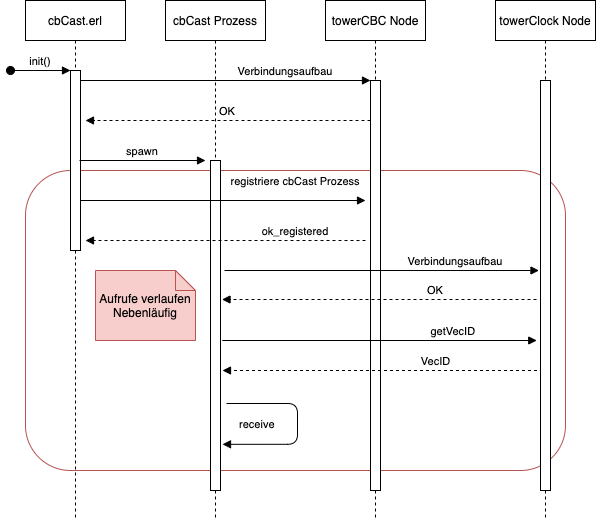
\includegraphics[scale=0.7]{Latex/Bilder/Sequenzdiagramm_cbCast.png}
\caption{\label{fig:sequence_cbCast} Sequenzdiagramm cbCast}
\end{center}
\end{figure}

Alternativ könnte sich der \textit{cbCast.erl} auch erst beim \textit{towerClock} die \textit{VektorID} holen und dann den \textit{cbCast} Prozess erzeugen. Durch den Ablauf in Abb. \ref{fig:sequence_cbCast} kann das holen der \textit{VektorID} aber nebenläufig zur Registrierung beim \textit{towerCBC} passieren. Der ganze Vorgang ist somit schneller.


\subsection{Vektoruhr Zentrale/Tower} \label{tower}

Die zentrale Vektoruhr (\textit{Tower}) verwaltet die Prozessnummern. Prozessnummern sind im Folgenden eindeutige IDs aus positiven ganzen Zahlen.

\subsection{TowerClock}

Der TowerClock implementiert eine wesentliche Schnittstelle, \textit{getVecID}. Aus Gründen der Erweiterbarkeit und Sicherheit mappt die TowerClock die Prozess ID des anfragenden Prozesses auf dessen Vektoruhr ID.
\\Die kleinste Zahl für eine Vektoruhr ID ist 0.

\subsection{Generelle Designentscheidungen}

\subsubsection{Logging}

Es wird pro Node eine generische .log Datei geben. Zum Beispiel für den Node \textit{'cbCast1@MacBook-Air-von-Kristoffer'} gibt es die Datei \textit{'cbCast1@MacBook-Air-von-Kristoffer'.log}. Dies bringt den Vorteil, dass die verschiedenen Kommunikationseinheiten - welche über die gleiche .beam Datei ausgeführt werden, aber auf verschiedenen Nodes laufen - separat voneinander geloggt werden.
\\Zum Debuggen war ein Gedanke, zusätzlich eine Logging Datei zu erstellen, in welcher alle Prozesse loggen. Hierdurch kann sequenziell nachverfolgt werden, ob die Reihenfolge der Aufrufe korrekt verläuft. Im Verlauf der Implementierung hat sich rausgestellt, dass diese Datei wenig Mehrwert bringt. Deswegen fehlt diese in der finalen Implementierung.